\chapter{Introduction}
\section{Introduction}

 Bacteria were one of the first life forms to appear on earth and have a profound and diverse impact on our lives \citep{abedon_bacteriophage_2008}.  It has been shown that the ratio of human cells to bacterial cells, in the human body, is close to 1:1 \citep{sender_revised_2016}, an update of the popular estimate that bacterial cells outnumber human cells in our body by the ratio 10:1 \citep{luckey_introduction_1970,savage_microbial_1977}. In 1915, the British microbiologist Fredrick Twort \citep{twort_investigation_1915} observed the phenomenon of clearing in a solution of bacteria and thought that it was caused by an enzyme responsible for killing bacteria \citep{weitz_quantitative_2017}. In 1917, the French physician Felix d’Herelle observed the same clearing phenomenon and speculated that an organism, which he called bacteriophage (phage for short) or “bacteria eater”, was responsible for killing the bacteria \citep{dHerelle_1917}. After the direct visualization of these bacteria eaters under the electron microscope, it was established that these bacteria eaters are organisms \citep {borries_bakterien_1938}, the bacteriophages.  Phages outnumber their bacterial hosts by a ratio of approximately 10:1 \citep{bergh_high_1989}, making them  the most abundant microorganisms in the biosphere \citep{rohwer_global_2003, clokie_phages_2011} and have been critical players in the evolutionary history of bacteria \citep{stern_phage-host_2011}. 

\section{Bacteriophages}
\subsection{Phage life cycle}
Although some viruses do not exclusively depend on their host for replication and carry with them genes needed for the processes thought to be the distinguishing characteristic of life \citep{raoult_1.2-megabase_2004}, most viruses require a host for their replication. A phage starts its life cycle by  attaching to a specific receptor on the surface of the bacterial host. Once attached, the phage injects its viral genome into the host cell. After injection, these viral genomes can take several possible pathways, of which the most well-known are:
(1) the viral genome takes over the host's cellular machinery, the viral genome is replicated and the structural components are produced, ultimately leading to the death of host cell and release of progeny virions into the environment, known as the lytic life cycle; and (2) the viral genome once inside the cell is integrated with the host bacterial genome, known as the lysogenic life cycle. 

 Phages that can follow only the lytic life cycle are called lytic phages whereas phages which follow either the lytic or lysogenic life cycle are called temperate phages. The majority of the identified temperate phages are double-stranded (ds) DNA viruses \citep{szekely_single-stranded_2016}, with the exception of a few single-stranded (ss) DNA temperate phages  \citep{krupovic_single-stranded_2015}. Integrated viral DNA of a temperate phage is referred to as a prophage and the bacterial cell carrying prophage or prophages is called a lysogen \citep{lwoff_lysogeny_1953}.  These prophage sequences are transmitted vertically with the genome of the bacterial host as the host cell divides into daughter cells \cite{feiner_new_2015}. 

 
 Since the discovery of phages, the ability of lytic phages to eradicate a bacterial population has been used to treat bacterial infectious diseases in humans, animals, and plants \citep{abedon_editorial:_2017,myelnikov_alternative_2018}.  After the advent of antibiotics to treat infectious diseases, phage therapy was confined to particular regions of the world \citep{myelnikov_alternative_2018}. Recently, due to the emergence of antibiotic-resistant bacteria, attention has been refocused on phage as a weapon against bacterial infectious diseases \citep{abedon_editorial:_2017, bull_dynamics_2002}. 
 
 \subsection{Bacterial genome sequencing}
Bacterial genomes are compact as compared to eukaryotic genomes in a sense that bacterial genomes contain less noncoding DNA, see Figure~\ref{fig:compact}.
Bacterial genomes vary in size by at least an order of magnitude \citep {bobay_evolution_2017} and may be up to 30 Mb in size \citep{brown_genomes_2007}. Bacterial genomes are dynamic and are exposed to various events dominated by insertions and deletions of genetic elements \citep{sela_theory_2016}. To understand the role of bacteria in shaping our environment and to eliminate various bacterial diseases, a complete understanding of the bacterial genome is important. 

The year 1995 is marked as the year when the first two human pathogenic bacterial genomes, \textit{Haemophilus influenzae} \citep{fleischmann_whole-genome_1995} and \textit{Mycoplasma genetalium} \citep{fraser_minimal_1995}, were sequenced. Since then bacterial genome sequencing has undergone substantial development. From 1995 – 2009 only 2010 sequenced bacterial genomes were submitted to NCBI, this number has increased with the advent of modern technologies  and 213,581 bacterial genomes have been sequenced and submitted to NCBI (as of November 2019), see Figure~\ref{fig:seqgenomes}.  
  The process of extracting biological information from sequenced bacterial genome data and providing descriptive information to these features is called bacterial genome annotation.
   \begin{figure}[t]
    \centering
     \begin{subfigure}[t]{0.45\textwidth} 
    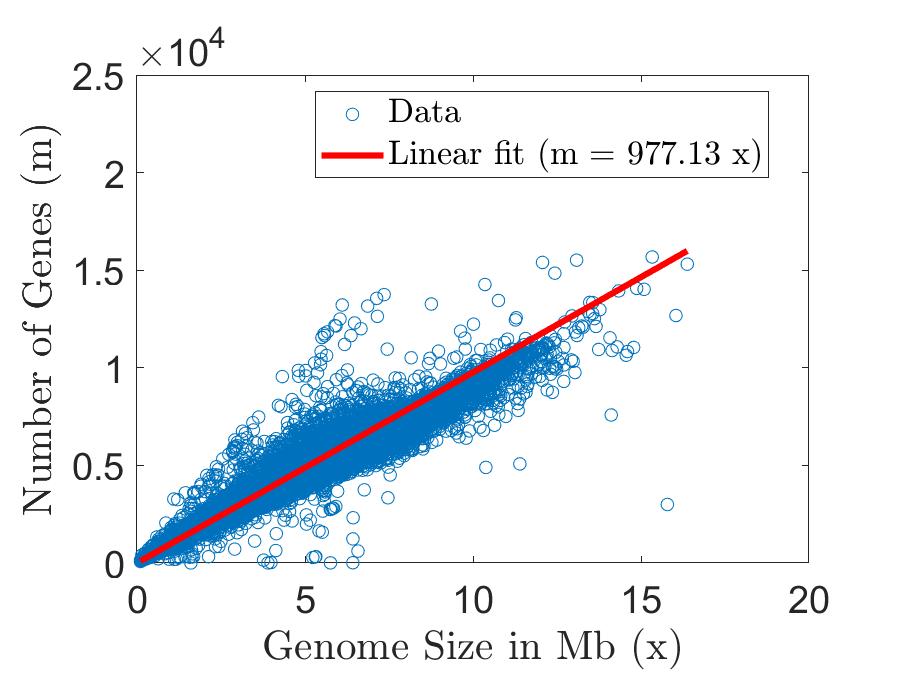
\includegraphics[scale=0.55]{bac}
     \subcaption{Number of genes versus bacterial genome size, showing a high correlation (correlation coefficient $r$ =0.984) between genome size and number of genes contained. }
     %\label{fig:brug_bar}
     \end{subfigure}\hfill
         \begin{subfigure}[t]{0.45\textwidth}
          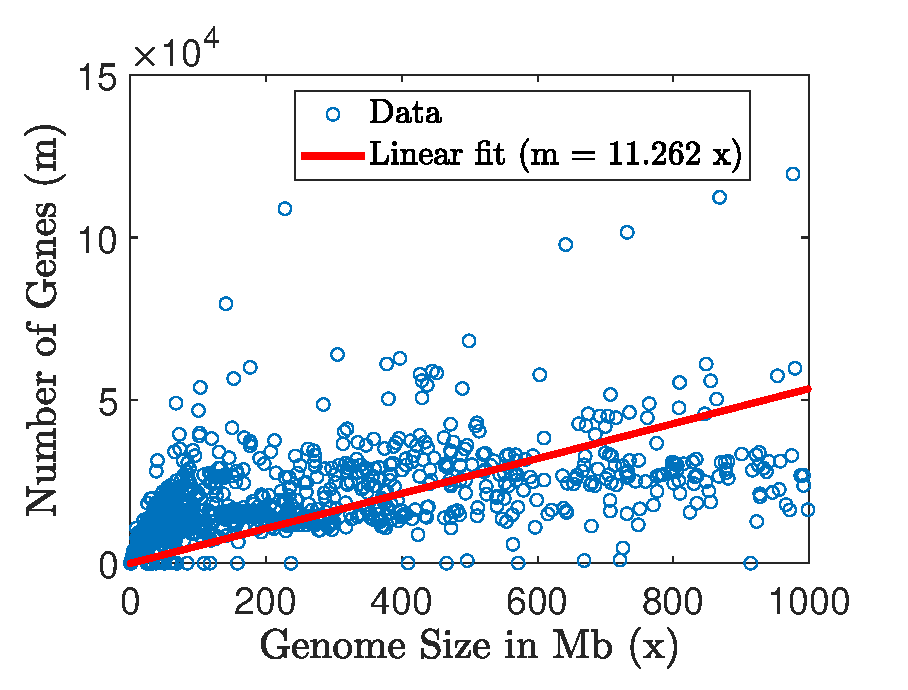
\includegraphics[scale=0.55]{eu}
            \subcaption[subfigcapskip = 50pt]{Number of genes versus eukaryotic genome size, showing a lower correlation ($r$ =0.624) between eukaryotic genome size and number of genes.}
            %\label{fig:}
    \end{subfigure}\hfill
    \caption[Prokaryotic genomes are compact as compared to eukaryotic genomes.]{Prokaryotic genomes are compact as compared to eukaryotic genomes. These data were downloaded from GenBank in November 2019 and consist of 190,618 bacterial genomes and 2,379 eukaryotic genomes.}
    \label{fig:compact}
\end{figure}
\begin{figure}[t]
    \centering
         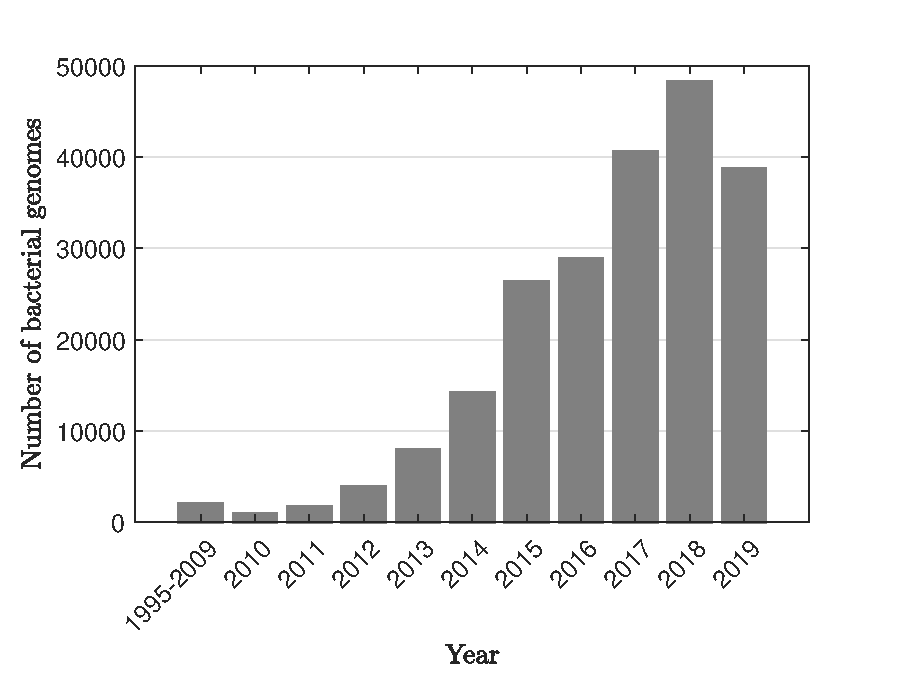
\includegraphics[scale=0.7]{bacseq}
         \caption[The number of bacterial genome sequences submitted to NCBI is growing rapidly.]{The number of bacterial genome sequences submitted to NCBI is growing rapidly. These data were downloaded from NCBI in November 2019.}
         \label{fig:seqgenomes}
\end{figure}
  \subsection{Prophage abundance and detection in bacterial genomes}
% [Be careful not to self-plagiarize.  None of the sentences in this section should be repeated in the introductory material of the later chapters.  Re-phrase here if they are the same sentences so that the papers can be inserted as chapters "as is".]
In the event of lysogeny, temperate phages can integrate their genome into different chromosomal sites of a bacterial genome. Phage $\lambda$ DNA integrates at a unique site in the bacterial genome \cite{tal_location_2014}, phage P2 integrates its genome at at least 10 different sites in the host bacterial genome \cite{barreiro_attachment_1992}, whereas phage Mu can integrate randomly into the host bacterial genome \cite{bukhari_random_1972}. Bacterial genome sequencing has revealed that prophages are not only frequently identified in pathogenic bacterial strains \citep{canchaya_impact_2004}, but are abundant in many bacterial genomes. Prophages may constitute up to 20\% of a bacterial genome \citep{casjens_prophages_2003}. The distribution of prophages in a bacterial genome is variable, ranging from no prophage to several prophages per bacterial genome  \citep{touchon_genetic_2016}. For example, the sequenced \textit{Escherichia coli} O157:H7 strain Sakai has been shown to contain 18 prophages which make up 16\% of its total genome content. 

Temperate phages, after integration with the bacterial genome, repress their lysis genes \citep{lawrence_where_2001} and are subject to mutations that are biased towards deletions \citep{casjens_prophages_2003}.  This mutational degradation may eliminate the ability of a prophage to enter into the lytic life cycle by deleting or damaging genes required for lysis and re-infection.  Prophages lacking the ability to enter into the lytic life cycle are called defective or cryptic prophages \cite{de_bruijn_prophages_1998}. It has been shown that defective prophages are abundant in bacterial genomes, for example, \textit{Escherichia coli} K-12 contains nine cryptic prophage elements in its genome \citep{wang_cryptic_2010}. 

A prophage, after insertion into the bacterial genome, becomes a part of the bacterial genome.  This relation between prophages and host bacterial cells is usually stable but intact prophage may initiate the lytic life cycle spontaneously \cite{ fothergill_effect_2011, james_differential_2012}, or in response to some environmental cues, or DNA damaging agents \cite{ barnhart_prophage_1976, lopez_induction_2014}, resulting in the killing of the host and release of progeny virions into the environment. This process is called the induction of a prophage and is very common in the bacterial world \cite{ alexeeva_spontaneously_2018}.  Some prophages, like $\lambda,$ excise from the bacterial chromosome to initiate the lytic life cycle, while others, like Mu, produce viral particles before excision from the host bacterial genome \citep{shapiro_molecular_1979}.

 Prophage sequences bring with them many genes, making prophage  a prominent source of genetic diversity within bacterial populations \cite{fortier_importance_2013}. Amongst the changes caused by prophages of particular interest has been the contribution of prophages to bacterial virulence and antibiotic resistance \cite{wagner_bacteriophage_2002,fortier_importance_2013, haaber_bacterial_2016}. 
 
Prophages can be identified in a bacterial genome using experimental or computational approaches. In the experimental approach, bacteria are usually exposed to UV light or other DNA-damaging conditions to cause the induction of prophages present in the bacterial genome. This technique clearly overlooks the presence of defective prophages as well as other prophages that could not induce.  Since a large number of sequenced bacterial genomes are publicly available, computational approaches to identify prophages are preferred.  

Since the early 2000s many computational approaches have been developed to find prophages in bacterial genomes. Different computational programs used to identify prophages include Dinucleotide abundance \citep{nicolas_mining_2002, srividhya_identification_2007}, Phage\_Finder \citep{fouts_phage_finder:_2006}, Prophage Finder \citep{bose_prophage_2006}, Prophinder \citep{lima-mendez_prophinder:_2008}, PHAST (PHAge Search Tool) \citep{zhou_phast:_2011}, PHASTER (PHAge Search Tool – Enhanced Release), an improved version of PHAST \citep{arndt_phaster:_2016},  PhiSpy \citep{akhter_phispy:_2012}, VirSorter \citep{roux_virsorter:_2015}, VRprofile \citep{li_vrprofile:_2017} and others. Using these computational tools it has been shown that prophages are abundant in bacterial genomes. PhiSpy \citep{akhter_phispy:_2012}, written in Python and C++, was used to identify 36,488 prophages from the analysis of over 11,000 bacterial genomes; 83\% of the bacterial genomes contained at least one prophage \citep{kang_prophage_2017}. In another study, PHAST \citep{zhou_phast:_2011} was used to identify 4122 prophages in 795 \textit{Acinetobacter baumannii} genomes, for an average of 5 prophages per bacterial genome \citep{costa_genomic_2018}. Of these prophages 78\% were identified as defective. Using PHASTER, Mottawea et al. were able to identify 11,297 prophages in 1760 \textit{Salmonella enterica} genomes \citep{mottawea_salmonella_2018}.

\subsection{Previous studies of phage-bacteria interaction}
Phages contribute to maintaining bacterial diversity \citep{buckling_role_2002}, alter competition between bacterial species \citep{bohannan_relative_2000} and mediate the exchange of genetic material among bacteria through horizontal gene transfer \citep{soucy_horizontal_2015, canchaya_prophage_2003}. Bacteria are constantly evolving to evade phage infection and phages are acquiring new strategies to infect their bacterial hosts; for details see \citep{rostol_phighting_2019, koskella_bacteriaphage_2014}. To elaborate the population dynamics of phage-bacteria interactions, both experimental and theoretical studies have been undertaken.


The population interaction between phages and bacteria in laboratory setting has been studied by many authors \citep{horne_coevolution_1970, levin_resource-limited_1977,lenski_constraints_1985, bohannan_effect_1997}. 
These studies have considered the interaction between \textit{E. coli} B with T2 phages and mixed species of bacteria with T2 and T3 phages. These investigations reported long-term coexistence of bacterial and viral populations in laboratory cultures. In 1977 Levin et al.  investigated the interaction between phages and bacteria by considering a culture of \textit{E. Coli} B (T2 sensitive) and K12 (T2 resistant) with virulent phage T2 \citep{levin_resource-limited_1977}.  Figure~\ref{fig:levin}  illustrates the results of \citep{levin_resource-limited_1977} and Figure~\ref{fig:levin2} illustrates the results of a related, later study  \citep{bohannan_effect_1999}.

\begin{figure}[t]
\begin{subfigure}[t]{0.45\textwidth}
\centering
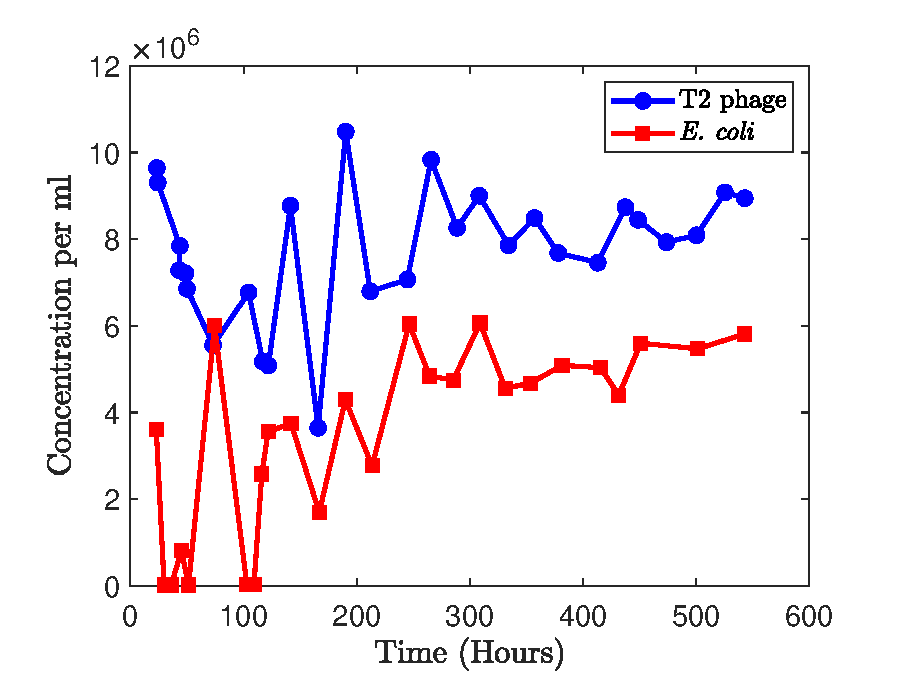
\includegraphics[scale=0.55]{L3.eps}
\subcaption[subfigcapskip = 50pt]{Density of glucose-limited populations with a T2-sensitive strain of \textit{E. coli} B and the bacteriophage T2.}

\end{subfigure}\hfill
\begin{subfigure}[t]{0.45\textwidth}
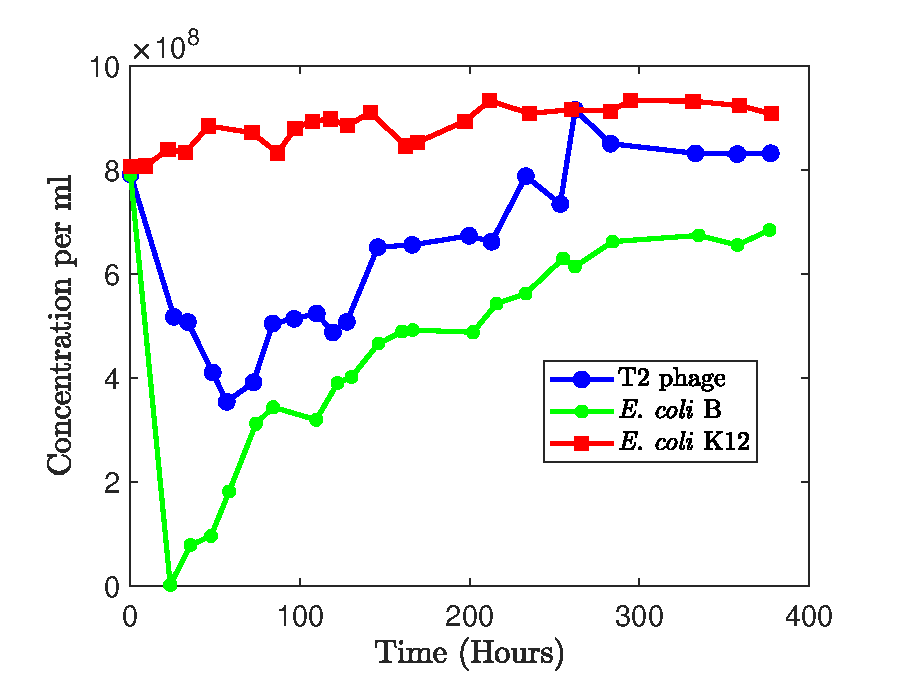
\includegraphics[scale=0.55]{L4.eps}
\subcaption[subfigcapskip = 50pt]{Glucose-limited continuous culture populations with a T2-sensitive strain of \textit{E. coli} B, a T2-resistant strain of \textit{E. coli} K12, and the bacteriophage T2.}
\end{subfigure}\hfill
\caption[Population dynamics of sensitive, resistant bacteria and virulent phage.]{Population dynamics of sensitive, resistant bacteria and virulent phage. These data were extracted from Figure 5A and Figure 8 of Levin et al. (1977) \cite{levin_resource-limited_1977}, using PlotDigitizer.}
\label{fig:levin}
\end{figure}
\begin{figure}[t]
\captionsetup[subfigure]{labelformat=empty}
\centering
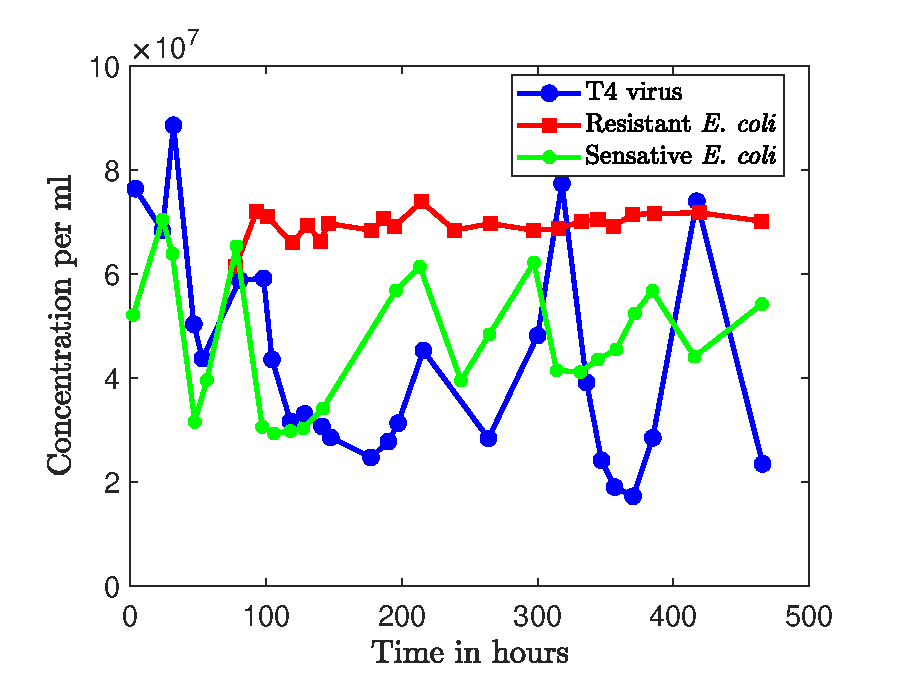
\includegraphics[scale=0.65]{L1.eps}
\caption[Dynamics of \textit{E. coli} and bacteriophage showing oscillating dynamics.]{Dynamics of T4 sensitive \textit{Escherichia coli} (green), T4 resistant \textit{Eschericia coli} (red), and bacteriophage T4 (blue) in chemostats supplied with media containing glucose, showing oscillating dynamics. Resistant \textit{E. coli} emerges approximately after 78 hours. The population of T4 phage and sensitive bacteria oscillate. The data was extracted from Figure 2B of Bohannan et al. (1999)  \cite{bohannan_effect_1999} using PlotDigitizer. }
\label{fig:levin2}
\end{figure}

In the Lotka-Volterra model, introduced by Lotka in 1925 \cite{lotka_elements_1925} and Volterra in 1926 \cite{volterra_variations_1928}, the consumption of prey follows the law of mass action, i.e. the consumption of prey by a predator is proportional to the product of the population density of predator and prey. The prey population grows exponentially in the absence of a predator, and the predator population declines exponentially in the absence of the prey.  The associated system of differential equations:   
\begin{eqnarray}\label{L-V}
\frac{dx}{dt} & =& r x - g x y \nonumber\\
\frac{dy}{dt} & = & \gamma g x y - \mu  y
\end{eqnarray}
gives the classical Lotka-Volterra model.  Here, $x$ corresponds to the population density of the prey, $y$ corresponds to the population density of predator, $r$ is the rate of increase of prey population, $g$ is the predation rate, $\gamma$ is the reproduction rate of predators and $\mu$ is the mortality rate of predators. With appropriate parameter values, this model predicts the coexistence of predator and prey, see Figure~\ref{fig:lotka}.

\begin{figure}[t]
\captionsetup[subfigure]{labelformat=empty}
\centering
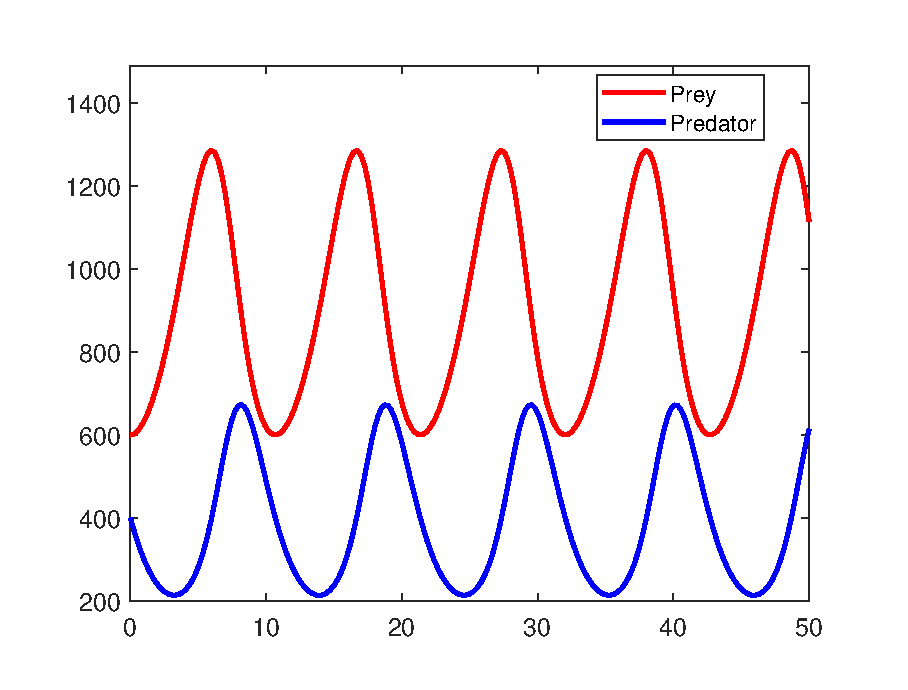
\includegraphics[scale=0.65]{lotka.eps}
\caption{Lotka-Volterra model showing long-term existence of both predator and prey populations.}
\label{fig:lotka}
\end{figure}

This model has been further improved, for example, by introducing a logistic growth term $r (1-\frac{x}{K})$, where $K$ is the carrying capacity of the prey population, instead of the exponential growth term $r x$ \cite{nisbet_modelling_1982}.  The linear functional response $ \mathcal{F}(x) =  g \,x$ in System \ref{L-V}, called the Holling Type I response, can also be replaced by more realistic functional responses (Holling Type II, Holling Type III and Holling Type IV) \citep{dawes_derivation_2013}.   

Based on the nature of the interaction between phages and bacteria and the qualitative behaviour of such predator-prey models, predator-prey type models were the natural choice for modelling the interaction between phages and bacteria. In 1961 Campbell \cite{campbell_conditions_1961} presented the following model 
\begin{eqnarray}\label{Camp}
\frac{dB}{dt} & =& r_{B} B \left(1-\frac{B}{K}\right) - aB -  k PB \nonumber\\
\frac{dP}{dt} &=& k b B(t-l) P(t-l) - k BP - a P - d P ,
\end{eqnarray}
where $B$ and $P$ are population densities of bacteria and free phages, respectively. The parameters $r_B$, $a$, $k$, $d$ represent the growth rate of bacteria, the flow rate constant, the absorption rate and the rate of spontaneous inactivation of phages, respectively.  Each infected bacterial cell yields $b$ phage particles (burst size) at a time $l$ seconds after infection. The author performed a local steady-state analysis of this model, concluding that phages will maintain bacteria at a low but non-zero level if they grow rapidly; otherwise phages will die out. In System \ref{Camp}, the functional response is $\mathcal{F} = k B$. 

Building on the Campbell model and to account for the relationship between prey growth and the availability of resources, a chemostat model with constant inflow of nutrient solution and outflow of culture was proposed by Levin et al. in 1977 \cite{levin_resource-limited_1977}. Multiple resources and multiple species of bacteria and phages were considered. Therefore, phages compete in addition to bacterial competition. The behaviour of the model developed was compared with that of experimental populations of \textit{E. coli} and its virulent virus T2, see Figure~\ref{fig:levin}. 

Campbell did not discuss the stability analysis at all, whereas Levin et al. investigated the model by integrating the equations numerically but did not carry out stability analysis analytically. Bremermann \cite{bremermann_parasites_1983} presented a relatively simpler model by assuming that time delays were negligible on the timescale of consideration. He did not use delay differential equations. If  $S$ denotes the density of susceptible hosts, $I$ denotes the density of infected hosts and $P$ the density of phages, then the equations for this model are given as:
\begin{eqnarray}\label{Br}
\frac{dS}{dt} &=& r_s S \left(1- \frac{S}{K}\right) - \beta S P \nonumber\\
\frac{dI}{dt} &=& \beta S P - \lambda I \nonumber\\
\frac{dP}{dt} &=& b I - \mu P.
\end{eqnarray}
Here $r_s$ is the bacterial growth rate, $K$ is its carrying capacity, $\beta$ is the rate of adsorption, $\lambda$ is the death rate of infected bacterial hosts, $b$ is the rate at which new phages are produced (burst size) and $\mu$ is the death rate of phages.  By carrying out stability analysis of  system \ref{Br} the author was able to show that the existence of phages depends on the carrying capacity of the bacteria, $K$. If the carrying capacity falls below a certain threshold $\left( \frac{\lambda\, \mu}{b\, \beta}\right)$ the phage population and infected hosts will die out and they uninfected host population will approach its carrying capacity $K$.  

Later, several authors modified the above models. For example Lenski et al. \cite{lenski_constraints_1985} included mutational events into the Levin et al. model \cite{levin_resource-limited_1977}. These authors also compared model predictions with the results of experiments with \textit{E. coli} and virulent phage and the evolutionary constraints for \textit{E. coli} and virulent phage.  In 1997, Bohannan and Lenski \cite{bohannan_effect_1997} model was a modification of the Levin model. This model ignored the dynamics of infected cells by considering them to instantaneously become dead. The authors solved the model analytically and examined the behaviour of the system numerically. The dynamics of the T4 and \textit{E. coli} populations were also shown, see Figure~\ref{fig:levin2}. A model, similar to Bremermann's model, was proposed by Beretta and Kaung  in 1998 \cite{beretta_modeling_1998} for marine bacteriophages. A rich literature about phage-bacteria interactions is now available, for detail see \cite{payne_understanding_2001, gourley_delay_2004, smith_models_2008}.  

\section{Mobile genetic elements}
Mobile Genetic Elements (MGEs) are DNA segments that encode enzymes or other proteins that mediate DNA movements within genomes or between bacterial cells \cite{frost_mobile_2005}. MGEs are involved in all aspects of genome organization, function, and evolution \cite{craig_mobile_2015, arkhipova_mobile_2016}. Horizontal gene transfer (HGT) is the intercellular movement of DNA that allows transfer of genes from one bacterium (donor) to another bacterium (recipient) by means other than vertical transmission. This transfer of genetic material can take place through: (1) transformation, where bacteria take DNA from their environment; (2) conjugation, where DNA is exchanged between two bacteria; or (3) transduction, which is bacteriophage-mediated exchange of genetic material between two bacteria \cite{soucy_horizontal_2015}. 
The role of HGT in bacterial evolution has long been recognised \cite{huddleston_horizontal_2014, soucy_horizontal_2015}.   
\subsection{Overview of mobile genetic elements}
The discovery of MGEs is attributed to McClintock for her work on the maize chromosome, where the existence of jumping genes in maize chromosomes was reported \cite{mcclintock_origin_1950}. The genomes of both prokaryotes and eukaryotes carry abundant MGEs \cite {schnable_b73_2009, lynch_origins_2007}. In this investigation, we will focus only on MGEs in prokaryotic genomes.  

MGEs can be categorized into different classes; we outline four important classes here. 
(1) Bacteriophages (lytic/lysogenic/prophages) are one of the most important classes of MGEs which help bacterial cells to exchange genetic material with each other through HGT \cite{ canchaya_phage_2003}. (2) Plasmids are extra-chromosomal genetic material and are very common in bacterial genomes \cite{ phillips_plasmid_2004}. Plasmids are transformed from donor bacterium to recipient bacterium through conjugation, a form of horizontal gene transfer in which bacteria exchange genetic material directly \cite{ phillips_plasmid_2004}.  Plasmids usually carry genes that bring genotypic changes to its bacterial host, for example, antibiotic resistance genes \cite{ svara_evolution_2011}.   
(3) Transposable elements (TEs) are ubiquitous DNA sequences in bacterial genomes that move within their host bacterial genome \cite{ garrido-ramos_evolutionary_2012}. 
(4) Insertion sequences (ISs), a type of TE \cite{capy_dynamics_1998}, are the simplest of MGEs and can move around within genomes or horizontally as a part of other MGEs \cite{ vandecraen_impact_2017}.

 \subsection{Evolutionary forces affecting mobile genetic elements}
 
 Mobile genetic elements are either intracellular (inserted from within the cell) or intercellular (inserted from another cell) and are typcically considered to be genetic parasites or junk DNA. The insertion of these new genetic materials comes with some cost to the bacterial host. The cost incurred by these MGEs to the host varies significantly and depends on the nature of the inserted element. Bacteriophages kill their host to release progeny virions but other mobile genetic elements like plasmids or TEs do not kill their host cell. However, to maintain these elements in its genome the host bacteria must exert some extra energy, making them costly \cite{diaz_ricci_plasmid_2000}.  These MGEs can also disrupt important functions by disrupting a bacterial gene upon insertion \cite{simser_novel_2005, naito_role_2016}.

On the other hand, these inserted genetic materials can also endow some benefits to their bacterial host by carrying genes that are beneficial to the host \cite{vandecraen_impact_2017}. Frost et al., in \cite{frost_mobile_2005}, called mobile genetic elements  ``the agents of open source evolution". 
Mobile genetic elements may also have a positive impact on the bacterial host’s neighbours by producing proteins that are beneficial for neighbours \cite{livermore_beta-lactamases_1995} or a negative impact by producing proteins that harm the host’s neighbours \cite{dykes_selection_1997}.  The relationship between mobile genetic elements and their host and host’s neighbours is further explained by  Rankin et al. in \cite{rankin_what_2011}.
 
 Once inserted into the bacterial genome, MGEs are faced with several evolutionary forces:
 
 (1) The rate of insertion of these MGEs into the bacterial genome is an important factor in determining their future distribution in the host population. For example, an important factor in determining the prophage distribution in bacterial genomes is the lysogeny \cite{bobay_pervasive_2014}, the integration of the phage genome with the bacterial genome after it enters into the bacterial cell.
 
(2) Mutation occurs randomly and is a change in the nucleotide sequence of a short region of a genome. Mutation is considered to be an important force in shaping bacterial genome evolution \cite{hershberg_mutationengine_2015}. It has been shown that mutation in the bacterial genome is biased toward deletion \cite{kuo_deletional_2009}.  Mutations have important and profound affects on these MGEs, for example, mutation can impair genes required for the excision of prophage from a bacterial genome, resulting in domestication of these prophages in bacterial genomes \cite{casjens_prophages_2003, wang_cryptic_2010}.

(3) MGEs, inserted into bacterial genomes, are part of the bacterial host genome and are transmitted vertically from parent to offspring. If these MGEs contain genes that can help its host to proliferate this will, in turn, help these MGEs to proliferate in the host population. 

(4) Many MGEs have the ability to invade host genomes horizontally. As described before, this horizontal transfer of genes between bacterial genomes is considered to be a very important factor in the evolution of bacterial genomes and may occur through conjugation, transformation or transduction  \cite{soucy_horizontal_2015}.

(5) MGEs usually have a stable relationship with their host's genome and are transmitted vertically as a part of the bacterial genome to the daughter cells. However some MGEs, like prophages, can excise from the bacterial genome, in response to environmental signals or spontaneously, and kill the host bacterium \cite{lopez_induction_2014}. 

\subsection{Mathematical modelling of mobile genetic elements}
Since the discovery of mobile genetic elements there have been many theoretical approaches to explain the nature of these DNA segments. Most of these approaches deal with a particular class of MGEs. The initial mathematical models of MGEs were mostly focused on understanding the mechanisms that prevent the unlimited expansion of MGEs in host populations, despite their tendency for proliferation. These studies also focused on obtaining the equilibrium copy number distribution under diverse evolutionary scenarios. Below we provide some overview of these models aimed at the evolution of MGEs in prokaryotic genomes.

Stewart and Levin, in 1977, developed an ODE model for the population dynamics of horizontally transmitted plasmids in bacterial genomes \cite{ stewart_population_1977} and argued that plasmids could not persist if there is a low rate of HGT. They also argued that if plasmids persist, then cells carrying them will maintain high frequencies in bacterial populations, even if the cells carrying them are less fit. In 1980, Levin and Stewart presented an ODE model for the population dynamics of nonconjugative plasmids \cite{levin_population_1980}. Here they concluded that nonconjugative plasmids could be maintained even when the bacteria carrying them have a lower reproduction rate than other bacteria and it is highly unlikely that they will be maintained without conferring to the host some selective benefit. The above mentioned models assume that random encounters occur between members of the plasmid-bearing population and plasmid-free population, at a rate that is proportional to the densities of these populations, that is, the law of mass action. Several variants of these models were presented over the years, for details see \cite{freter_experimental_1983, lundquist_transitory_1986, zhong_accounting_2010, turner_tradeoff_1998}. To capture the dynamics of the plasmid in spatially structured habitats other techniques have been applied, for example, computational models \cite{ krone_modelling_2007, lagido_model_2003, ponciano_population_2007, merkey_growth_2011, connelly_modeling_2011}.

The evolution of TEs in prokaryotic genomes has been studied by many authors \cite{hartl_why_1988, basten_branching-process_1991, moody_branching_1988, dolgin_fate_2006, wagner_cooperation_2006, drakos_extinction_2015, rabbani_dynamics_2016}. All these authors used the branching process method to study the evolution
of TEs in prokaryotic genomes.  In a Markov process the outcome of a state is independent of past states and depends only on the present state.  A branching process is a special type of Markov process. Using these methods, Sawyer and Hartl, in 1986, developed a model for the distribution of TEs in prokaryotic genomes \cite{sawyer_distribution_1986}. The model assumed that TEs are entering prokaryotic genomes at a constant rate and can reduce the fitness of the host in proportion to their numbers in the host genome. A model in which the TEs can convey a selective advantage to the host was also considered. The equilibrium distributions of copy numbers for these models were determined. Relevant parameters were estimated using data regarding the distribution of insertion sequences in natural isolates of \textit{Escherichia coli}. In another study, Hartl and Sawyer (1988) used a branching process to model the insertion sequences in \textit{E. coli} and concluded that horizontal gene transfer is essential in maintaining bacterial insertion sequences \cite{hartl_why_1988}. 

Basten and Moody formulated a model to analyze the spread of transposable genetic elements in prokaryotic genomes, in 1991 \cite{basten_branching-process_1991}.  The authors incorporated selection, transposition and deletion in their model. They concluded that TEs can spread through a population despite selection against them. In \cite{edwards_transiently_2003}, the effect of  a fluctuating environment on the spread and persistence of TEs was studied.  

Van Passel et al. developed a birth–death–diversification model for mobile genetic elements subject to sequence diversification \cite{van_passel_birth_2014}. They applied the model to putative mobile promoters, a type of MGE,  and quantified the relative importance of duplication, loss, horizontal gene transfer (HGT), and diversification to the maintenance of the PMP reservoir.

Finally, in 2018, Iranzo and Koonin developed an ODE model and carried out comparative genomic study to explain the roles of selection, horizontal gene transfer, gene duplication and gene loss in the spread and persistence of MGEs \cite{iranzo_how_2018}. By quantifying the fitness of MGEs to the bacterial hosts they showed that these MGEs are deleterious at evolutionary timescales and characterized them as parasites. 

\section{Motivation and outline of the thesis}
Due to the alarming spread of antibiotic resistance and its consequences to public health, the evolution of antibiotic resistance genes has been a topic of interest for many scientists \cite{ hong_comprehensive_2018}. Experimental results have shown that the synergistic use of antibiotics and phages has a promising effect against antibiotic resistance bacteria, especially those in biofilms \cite{chaudhry_synergy_2017}. In \textbf{Chapter 2}, we have developed an ODE model to study the effect of antibiotics and phages on the bacterial population in a biofilm. We have exploited the idea of a group defense mechanism by assuming that as the biofilm becomes more and more mature, the harder it becomes for phages to kill bacteria in the biofilm colony. Here we show that the synergistic use of phages and antibiotics, especially using phages first and then antibiotics, can incur maximum damage to the biofilm bacteria. We also show that neither phages nor antibiotics, alone,  can eliminate the biofilm completely. Complete elimination of biofilm bacteria is possible only if we could stop the further attachment of planktonic bacteria to the biofilm colony.

The advent of modern technologies has resulted in huge databases about MGEs and has opened new ways to investigate the evolution of MGEs and their role in the evolution of bacteria. Although a substantial literature is available about the evolution of MGEs, these studies are lacking the evolution of an important player responsible for the evolution of bacterial genomes and hence antibiotic resistance genes, the prophages. In \textbf{Chapter 3} we attempted fill this void. Here, we have developed a PDE model to mimic the prophage size distribution in bacterial genomes. The basic question we investigate here is \textit{``Why is the prophage size distribution in bacterial genomes bimodal?"} We fitted our PDE model to the three publicly available data sets and were able to quantify various evolutionary forces acting on prophages. 

The next question we investigated is \textit{``Which genes are enriched in defective prophages?".} In \textbf{Chapter 4}, we study the genetic repertoire of prophages, especially, which genes are enriched in defective prophages. We downloaded data describing prophages in two well-studied data sets from GenBank and examine their genetic repertoires. Here we developed an ODE model to investigate possible steady states of prophages genes. We also developed a gene-level model to get more insight into the genetic repertoire of prophages. 

In \textbf{Chapter 5}, we present conclusions and possible future work.  

\addcontentsline{toc}{chapter}{Bibliography}
\bibliographystyle{abbrv}
\bibliography{refrence}

